\documentclass[12pt]{report}
\usepackage[left=2cm,right=2cm,top=2cm,bottom=2cm]{geometry} % page settings
\usepackage[dutch]{babel} % provides dutch alternatives for english text
\usepackage[utf8]{inputenc} % provides UTF-8 encoding
\usepackage{color} % more color options
\usepackage{enumitem} % options for enumerations
\usepackage{amsmath} % provides many mathematical environments & tools
\usepackage{graphicx} % for displaying images

%DOCUMENT INFORMATION
\title{Samenvatting Statistiek}
\author{Bert De Saffel}
\date{2017-2018}

% CUSTOM COMMANDS
\setlength{\parindent}{0mm}
\graphicspath{{./img/}}
\newcommand{\todo}[1]{
  {\color{red}\textunderscore{\textit{TODO: #1}}}
}
\newcommand{\exercise}[2]{
  #1
  

  \underline{Oplossing}
  
  #2
  
    \hrulefill
}
\newcommand{\example}[2]{
      \hrulefill
      
      Voorbeeld: #1
      
      #2
      
      \hrulefill
  }

\begin{document}
\maketitle
\tableofcontents

\part{Theorie}
\chapter{Kansrekenen}
De kans op een gebeurtenis A:
$$P(A) = \frac{\hbox{\# gunstige gevallen}}{\hbox{tot \# mogelijkheden}}$$
Altijd geldig: 
$$0 \leq P(A) \leq 1$$
\section{Bewerkingen}
\begin{enumerate}
	\item $P(A \cap B)$: kans op gebeurtenis A en gebeurtenis B
	\item $P(A \cup B)$: kans op gebeurtenis A of gebeurtenis B
	\item $P(A|B)$: Voorwaardelijke kans (lees: Wat is de kans op A indien B waar is). A en B zijn onafhankelijk indien $P(A|B) = P(A)$ of $P(B|A) = P(B)$
\end{enumerate}
\section{Rekenregels}
\begin{enumerate}
	\item Optellingswet: $P(A \cup B) = P(A) + P(B) - P(A \cap B)$
	\item Vermenigvuldigingswet: $P(A \cap B) = P(A)P(B)$
	\item Complementswet: $P(\overline{A}) = 1 - P(A)$
	\item $P(A \cap \overline{B}) = P(A) - P(A \cap B)$
\end{enumerate}
\example{Wat is $P(A\cup B\cup C)$?}
{
	\begin{equation*}
		\begin{split}
			& P(A\cup B\cup C)\\
			= & P(A\cup B) + P(C) - P[(A \cup B) \cap C]\\
			= & P(A) + P(B) - P(A\cap B) + P(C) - P[(A \cap B) \cup (B \cap C)]\\
			= & P(A) + P(B) + P(C) - P(A \cap B) - [P(A \cap C) + P(B \cap C) - P(A \cap B \cap C)]\\
			= & P(A) + P(B) + P(C) - P(A \cap B) - P(A \cap C) - P(B \cap C) + P(A \cap B \cap C)
		\end{split}
	\end{equation*}
}



\section{Combinatieleer}
De permutatie(volgorde is van belang): $$P_n = n!$$ (Op hoeveel verschillende manieren kunnen we 5 studenten plaatsen op 5 stoelen \textbf{OF} het aantal verschillende manieren om \textit{n} elementen te ordenen)


De combinatie(volgorde is niet van belang): $$C_n^p = (_p^n) = \frac{n!}{p!(n - p)!}$$ (Op hoeveel verschillende manieren kunnen we 2 studenten kiezen uit 5 \textbf{OF} het aantal verschillende manieren om \textit{p} elementen te kiezen uit \textit{n}.)

\example{In een vaas zitten 8 rode, 4 witte en 3 blauwe knikkers. Wat is de kans om met trekken met teruglegging exact 2 rode knikkers te nemene bij het trekken van 5 knikkers?}{
	$$P(2R) = \frac{8}{15} \cdot \frac{8}{15} \cdot \frac{7}{15} \cdot \frac{7}{15} \cdot \frac{7}{15} \cdot C_5^2$$
	
	Het getal $\frac{8}{15}$ stelt de kans voor om een rode knikker te trekken. Het getal $\frac{7}{15}$ stelt de kans voor om geen rode knikker te trekken. Er wordt vermenigvuldigt met $C_5^2$ de 2 rode knikkers elk van de 5 plaatsen kunnen innemen.
	$$=C_5^2 \bigg(\frac{8}{15}\bigg)^2\bigg(\frac{7}{15}\bigg)^3$$
	$$= 10 \cdot \frac{64}{225} \cdot \frac{343}{3375} = 0.29 = 29\%\; \hbox{kans}$$
	
}

\section{Regel van Bayes}
$$P(A_j|B) = \frac{P(A_j \cap B)}{P(B)} = \frac{P(A_j)P(B|A_j)}{\sum_{i = 1}^{n}P(A_i)P(B|A_i)}$$

\example{In een jaszak zitten 2 munten: één normaal(N) en één vervalst(V) (munt aan elke zijde). Een muntstuk wordt aselect gekozen en gegooid. Munt komt bovenaan te liggen. Wat is de kans dat dit het normale muntstuk is? Dit muntstuk wordt opnieuw gegooid. Terug munt. Wat is nu de kans dat dit het normale muntstuk is?}{
	
	$$P(N) = \frac{1}{2}$$
	$$P(V) = \frac{1}{2}$$
	\\
	De kans dat het munt of kop is bij het normale muntstuk is 0.5.
	$$P(M/N) = P(K/N) = \frac{1}{2}$$
	De kans dat het munt is bij het valse muntstuk is 1.
	$$P(M/V) = 1$$
	Regel van Bayes:
	\begin{equation*}
	 \begin{split}
	  P(N/M) & = \frac{P(N)P(M/N)}{P(M/N)P(N) + P(M/V)P(V)}\\
	         & = \frac{\frac{1}{2} \cdot \frac{1}{2}}{\frac{1}{2} \cdot \frac{1}{2} + 1\cdot \frac{1}{2}}
	          = \frac{\frac{1}{4}}{\frac{3}{4}}
	          = \frac{1}{3}
	 \end{split}
	\end{equation*}
	Indien muntstuk opnieuw wordt gegooid:
	\begin{equation*}
	 \begin{split}
	   P(N/2M) & = \frac{P(N)P(2M/N)}{P(2M/N)P(N) + P(2M/V)P(V)}\\
	           & = \frac{\frac{1}{2} \cdot (\frac{1}{2} \cdot \frac{1}{2})}{(\frac{1}{2} \cdot \frac{1}{2}) \cdot \frac{1}{2} + 1\cdot \frac{1}{2}}\\
	           & = \frac{\frac{1}{4}}{\frac{5}{4}} = \frac{1}{5}
	 \end{split}
	\end{equation*}
}

\chapter{Beschrijvende statistiek}
\section{Populaties en steekproeven}
\begin{itemize}
	\item \textbf{Populatie}: Een verzameling van elementen 
	\item \textbf{Steekproef}: Een deelverzameling van de populatie. Deze moet representatief zijn (bv $3/4$ van de populatie is vrouw. In de steekproef moet ook $3/4$ vrouw zijn)
\end{itemize}
\section{Veranderlijken}
\begin{itemize}
	\item {\textbf{Stochastische variabele}: Kan waarden aannemen elk met een bepaalde kans.}
	\item {\textbf{Kwalitatieve variabele}: Geen numerieke waarden (bloedgroep, studierichting)}
	\item {\textbf{Kwantiatieve variabele}: Numerieke waarden (gewicht, leeftijd)}
	\item {\textbf{Ordinale variabele}: Er kan een bepaalde orde toegekend worden (zeer goed, goed, matig, voldoende, slecht en zeer slecht)}
	\item {\textbf{Nominale variabele}: Er kan geen bepaalde orde toegekend worden (studierichting)}
	\item {\textbf{Onafhankelijke variabele}: De ene meting beïnvloed de andere niet (gooien van een dobbelsteen)}
	\item {\textbf{Afhankelijke variabele}: De ene meting beïnvloed de andere (grootte per geslacht)}
	\item {\textbf{Discrete variabele}: Heeft enkel discrete waarden (1, 0.4, 7, 9 , 1/100)}
	\item {\textbf{Continue variabele}: Heeft continue waarden ($\sqrt{2}$, $[-10, 10]$)}
\end{itemize}
\section{Discrete veranderlijken}
\subsection{Ordenen van gegevens}
Stel \textit{n} het aantal elementen van de populatie of van een steekproef en \textit{k} het aantal verschillende waarden dat de veranderlijke kan aannemen.
$$\sum_{i=1}^{k} n_i = n$$
\begin{itemize}
	\item {\textbf{Absolute frequentie}: Het aantal keer dat een bepaalde waarde aangenomen wordt.
			
	}
	\item {\textbf{Relatieve frequentie}: De verhouding van de absolute frequentie tot het aantal elementen
		$$f_i = \frac{n_i}{n}\;\;\;\hbox{en}\;\;\;\sum_{i = 1}^{k} f_i = 1$$
	}
	\item {\textbf{Cumulatieve absolute frequentie}: 
		$$N_i = \sum_{j=1}^{i} n_j$$
	}
	\item {\textbf{Cumulatieve relatieve frequentie}:
		$$F_i = \sum_{j=1}^{i} f_i$$
	}
	\item {\textbf{Frequentietabel}: Voorstelling van alle frequenties.\\
		Een toets bij 204 studenten, gequoteerd op 10, leverde volgende resultaten:\\
		\begin{tabular}{l | l l l l l l l l l}
			score & 2 & 3 & 4  & 5  & 6  & 7  & 8  & 9  & 10 \\
			\hline
			$n_i$ & 1 & 5 & 16 & 21 & 39 & 44 & 50 & 26 & 2  
		\end{tabular}\\
		De frequentietabel wordt:\\
		\begin{tabular}{l | l | l | l | l | l | l | l | l | l}
			score & 2     & 3     & 4     & 5     & 6     & 7     & 8     & 9     & 10   \\
			\hline
			$n_i$ & 1     & 5     & 16    & 21    & 39    & 44    & 50    & 26    & 2    \\
			$f_i$ & 0.005 & 0.025 & 0.078 & 0.103 & 0.191 & 0.216 & 0.245 & 0.127 & 0.01 \\
			$N_i$ & 1     & 6     & 22    & 43    & 82    & 126   & 176   & 202   & 204  \\
			$F_i$ & 0.005 & 0.029 & 0.108 & 0.211 & 0.402 & 0.618 & 0.863 & 0.990 & 1    
		\end{tabular}
	}
\end{itemize}
\subsection{Plaatsparameters en spreidingsparameters}
\begin{itemize}
	\item {\textbf{Steekproefgemiddelde}: De som van alle waarnemingen gedeeld door het totaal aantal waarnemingen
		$$\overline{x} = \frac{1}{n}(x_1 + x_2 + ... + x_n) = \frac{1}{n} \sum_{i = 1}^{n} = x_i$$
	}
	\item {\textbf{Modus}: De waarde met de grootste absolute frequentie.}
	\item {\textbf{Mediaan}: Na orderning van de waarnemingen, de middelste waarde als n oneven is en het gemiddelde van de middelste twee als n even is.}
	\item {\textbf{Variantie}: Het rekenkundig gemiddelde van de \textbf{kwadraten van de afwijkingen} van de waarnemingsgetallen ten op zichte van hun rekenkundig gemiddelde:
		$$s^2 = \frac{1}{n - 1}\sum_{i=1}^{n}(x_i - \overline{x})^2$$}
	\item {\textbf{Standaardafwijking}: De vierkantswortel uit de steekproefvariantie. 
		$$\sigma = \sqrt{s^2} = s$$}
\end{itemize}
\section{Continue veranderlijken}
\subsection{Ordenen van gegevens}
Het ordenen van continue veranderlijken wordt gedaan met klassen.
\begin{itemize}
	\item {\textbf{Spreidingsbreedte (range)}: Het verschil tussen het grootste en het kleinste waarnemingsgetal.}
	\item {\textbf{Aantal klassen}: Het aantal klassen is de vierkantswortel uit het aantal elementen: $$k = \sqrt{n}$$}
	\item {\textbf{Klassebreedte ($\Delta x$)}: De breedte van elke klasse. Indien elke klasse een verschillende breedte heeft wordt $\Delta x_i$ gebruikt om de \textit{i}-de klasse aan te duiden.}
	\item {De frequenties zijn analoog aan discrete veranderlijken}
\end{itemize}

\subsection{Plaatsparameters en spreidingsparameters}
\begin{itemize}
	\item {\textbf{Het rekenkundig gemiddelde}: 
		$$\overline{x} = \frac{1}{n}\sum_{i=1}^{k}n_ic_i$$
		met $c_i$ het klassemidden van de \textit{i}-de klasse.
	}
	\item {\textbf{De modale klasse}: De klasse met de grootste absolute frequentie.}
	\item {\textbf{De mediale klasse}: De klasse met de laagste waarden waarin de cumulatieve relatieve frequentie minstens 0.5 bedraagt}
	\item {\textbf{De variantie}:
		$$s^2 = \frac{1}{n-1}\sum_{i=1}^{k}n_i(c_i-\overline{x})^2$$
	}
	\item {\textbf{Standaardafwijking}:
		$$\sigma = \sqrt{s^2} = s$$}
\end{itemize}

\subsection{Momenten van een steekproef}
\todo{epic}

\chapter{verdelingsfuncties van een populatie}
Twee soorten verdelingsfuncties:
\begin{itemize}
	\item Kansfunctie: bij discrete kansen (sommeren)
	\item Dichtheidsfunctie: bij continue kansen (integreren)
\end{itemize}
\section{Kansfunctie}
De kansfunctie $f(x)$:
$$f(x_i) = P(X = x_i) \qquad \hbox{met}\qquad i = 1, 2, ..., k$$
$$f(x) = 0 \qquad \hbox{als} \qquad k \notin \{x_1, ..., x_n\}$$
De som van alle kansen is gelijk aan 1:
$$\sum_{i = 1}^{k} f(x_i) = 1$$
De cumulatieve distributiefunctie wordt gegeven door:
$$F(x) = P(x \leq t) = \sum_{x_i \leq t} f(x_i)\;dx$$
\section{Dichtheidsfunctie}
De som van alle kansen is gelijk aan 1:
$$\int_{-\infty}^{+\infty} f(x)\;dx = 1$$
Aangezien we integreren:
$$\int_{a}^{a} f(x)\;dx = 0$$
Hieruit volgt:
\begin{equation*}
	\begin{split}
		& P(a \leq x \leq b) \\
		= & P(a < x \leq b)  \\
		= & P(a < x < b)     \\
		= & P(a \leq x < b)
	\end{split}
\end{equation*}
De cumulatieve distributiefunctie wordt gegeven door:
$$F(x) = P(x \leq t) = \int_{-\infty}^{t} f(x)\;dx$$
\example{Stel $f(x) = 
	\begin{cases} 
		a + b(x - 1)^2  & 0 \leq x \leq 2
		               \\ 0 &  anders 
		
	\end{cases}$.\\ 
	Bepaal a en b zodat f een geldige dichtheidsfunctie is. Bepaal ook $F(t)$.}{
	
	\begin{equation*}
		\begin{split}
			\int_{-\infty}^{+\infty} f(x)\; dx = 1 
			& \Leftrightarrow \int_{0}^{2} a + b(x - 1)^3 \; dx = 1 \\
			& \Leftrightarrow ax + b\frac{(x - 1)^4}{4}\bigg|_{0}^{2} = 1 \\
			& \Leftrightarrow 2a + \frac{b}{4}(1 - 1) = 2 \\
			& \Leftrightarrow a = \frac{1}{2}
		\end{split}
	\end{equation*}
	
	Is $f(x) \geq 0\;\forall\;x$?
	\\
	Is $\frac{1}{2} + b(x - 1)^3 \geq 0$? $(x \in [0, 2])$
	$$\Rightarrow x \in [0, 2] \Rightarrow -1 \leq (x - 1)^3 \leq 1$$
	
	\underline{Als $b > 0$:}
	$$- b \leq b(x-1)^3 \leq b$$
	$$\frac{1}{2} - b \leq b(x-1)^3 + \frac{1}{2} \leq b + \frac{1}{2}$$
	$f(x)$ zal $\geq 0$ indien $\frac{1}{2} - b \geq 0$
	$$\Rightarrow b \leq \frac{1}{2}$$
	
	\underline{Als $b < 0$:}
	\begin{equation*}
		\begin{split}
			- b \geq b(x-1)^3 \geq b & \Rightarrow b \leq b(x-1)^3 \leq -b \\
			& \Rightarrow b + \frac{1}{2} \leq b(x-1)^3+ \frac{1}{2}  \leq -b + \frac{1}{2}
		\end{split}
	\end{equation*}
	$f(x)$ zal $\geq 0$ indien $\frac{1}{2} + b \geq 0$
	$$\Rightarrow b \geq -\frac{1}{2}$$
	
	\begin{equation*}
	 \begin{split}
	  F(t) & = \int_{0}^{t} \frac{1}{2} + b(x - 1)^3\; dx \;\; (t \in [0, 2])\\
	       & = \frac{1}{2}x + b\frac{(x-1)^4}{4}\bigg|_{0}^{t} \\
	       & = \frac{1}{2}t + \frac{b}{4}[(t-1)^4 - 1]
	 \end{split}
	\end{equation*}
	Bovendien is $F(t) = 0$ als $t < 0$ en is $F(t) = 1$ als $t > 2$
	
}

\section{Plaatsparameters}
Van een variabele x kennen we de dichtheidsfunctie $f(t)dt$ die de kans epaalt dat x een waarde in het interval $[t, t + dt]$ aanneemt. Voor een willekeurige functie $g(x)$ defineert men de verwachte waarde als volgt:
\begin{itemize}
 \item Discreet: $$E[g(x)] = \sum_{i = 1}^{k} g(x_{i})f(x_i)$$
 \item Continu: $$\int_{-\infty}^{+\infty}g(x)f(x)\; dx$$
\end{itemize}


\example{Wat is de gemiddelde waarde bij het gooien van een dobbelsteen}{
  \begin{equation*}
   \begin{split}
    \mu & = 1\cdot\frac{1}{6} + 2\cdot\frac{1}{6} +3\cdot\frac{1}{6} +4\cdot\frac{1}{6} +5\cdot\frac{1}{6}+ 5\cdot\frac{1}{6}\\
    &= 3.5
   \end{split}
  \end{equation*}
}
\example{Bepaal de gemiddelde winst als bij kop 3 euro wordt betaald en bij munt 5 euro. Het munstuk is vervalst zodat P(k) = 2P(M)}{
We maken een stelsel op met 2 formules. De extra formule is de som van alle kansen die gelijk is aan 1.
$$\begin{cases}
   P(K) = 2P(M) \\
   P(K) + P(M) = 1
  \end{cases}
$$
Hieruit wordt afgeleid dat 
\begin{equation*}
 \begin{split}
   P(K) &= \frac{2}{3} \\
   P(M) &= \frac{1}{3}
 \end{split}
\end{equation*}
De winstfunctie wordt gedefinieerd als g met g(K) = 3 en g(M) = 5.
\begin{equation*}
 \begin{split}
  E[g(x)] & = g(K)\cdot P(K) + g(M)\cdot P(M)\\
          & = 3 \cdot \frac{2}{3} + 5 \cdot \frac{1}{3}\\
          & = 2 + \frac{5}{3}\\
          & = \frac{11}{3}
 \end{split}
\end{equation*}
}
\example{Bereken de gemiddelde winst x met F(x) zoals grafisch weergegeven 
\begin{center}
 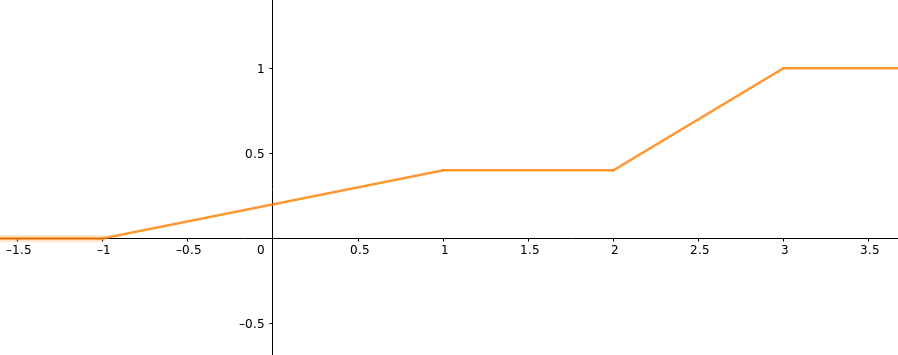
\includegraphics[width=0.5\linewidth]{slide_7}
\end{center}

}{
\begin{equation*}
 \begin{split}
  \mu & = E[x] \\
      & = \int_{-1}^{1} x\cdot f(x)\; dx + \int_{2}^{3} x\cdot f(x)\; dx
 \end{split}
\end{equation*}
De functie kan gedefinieerd worden als:
$$F(x) = \begin{cases}
   0.2(x + 1) & x \in [-1,1] \\
   1 + 0.6(x-3) & x \in [2,3] \\
   0 & x < -1 \\
   1 & x > 3 \\
   0.4 & x \in [1, 2]
\end{cases}$$
We weten dat $f(x) = \frac{dF(x)}{dx}$. We leiden $F(x)$ af voor de intervallen $[-1, 1]$ en $[2, 3]$ 
\begin{equation*}
      \begin{split}
       \mu & = \int_{-1}^{1} x\cdot \frac{1}{5}\; dx + \int_{2}^{3} x\cdot \frac{3}{5}\; dx \\
           & = \frac{x^2}{10}\bigg|_{-1}^{1} + \frac{3x^2}{10}\bigg|_{2}^{3} \\
           & = \frac{1}{10}\bigg[(1 - 1) + 3(9 - 4)      \bigg] \\
           & = \frac{15}{10} = \frac{3}{2}
      \end{split}
\end{equation*}
}
\example{Bereken de mediaan van x
\begin{center}
 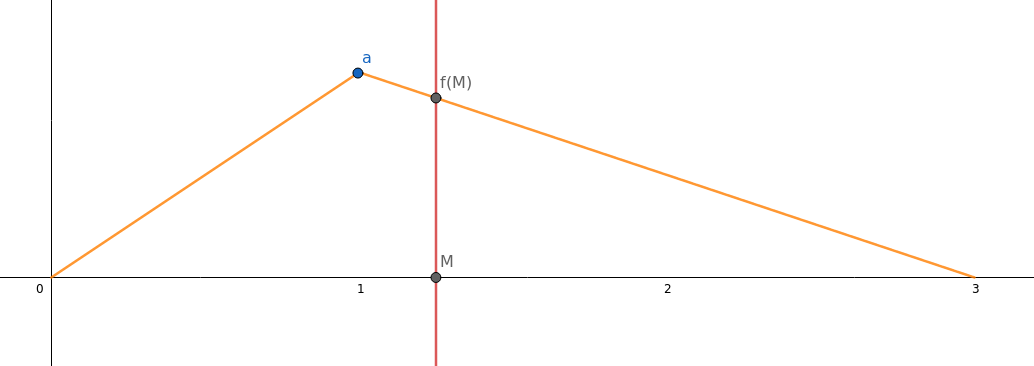
\includegraphics[width=0.90\textwidth]{oef_mediaan}
\end{center}
}{
De oppervlakte van het rechterdeel moet gelijk zijn aan 50\%. We gebruiken de formule van de oppervlakte van een driehoek.

\begin{equation*}
 \begin{split}
  &  \frac{(3 - M) \cdot f(M)}{2} = \frac{1}{2} \\
  \Leftrightarrow & (3 - M) \cdot f(M) = 1
 \end{split}
\end{equation*}
De som van alle kansen moet gelijk zijn aan 1.
\begin{equation*}
 \begin{split}
  \int_{0}^{3}f(x)\;dx = 1 & \Leftrightarrow \frac{a}{2} + a = 1\\
  & \Leftrightarrow a = \frac{2}{3}
 \end{split}
\end{equation*}
De rechte door $(2, \frac{2}{3})$ en $(3, 0)$ wordt gegeven door 
$$y = -\frac{1}{3}(x-3)$$
Herschrijf:
$$f(M) = -\frac{1}{3}(M - 3)$$
Nu kan de formule van de oppervlakte van de driehoek terug gebruikt worden:
\begin{equation*}
 \begin{split}
  & (3 - M)(-\frac{1}{3}(M - 3)) = 1  \\
  \Leftrightarrow & M = 3 \pm \sqrt{3}\\
  \Leftrightarrow & M = 3 - \sqrt{3} \;\;\;\hbox{(aangezien de functie niet hoger gaat dan 3)}
  \end{split}
\end{equation*}
}

\section{Spreidingsparameters}
De variantie:
\begin{itemize}
 \item \textbf{Continu}: $$\sigma^2 = V[x] = \int_{-\infty}^{+\infty}(x-\mu)^2 f(x)\; dx$$
 \item \textbf{Discreet}: $$\sigma^2 = V[x] = \sum_{i}(x_i - \mu)^2 f(x_i)$$
\end{itemize}
De standaardafwijking blijft $\sigma = \sqrt{\sigma^2}$

\example{Bewijs $V[ax + b] = a^2V[x]$}{
We bewijzen enkel voor een continue dichtheidsfunctie, maar is analoog aan discrete kansfuncties.

\begin{equation*}
 \begin{split}
  V[ax + b] & = \int_{-\infty}^{+\infty}(ax + b - a\mu + b)^2 f(x)\; dx \\
            & = \int_{-\infty}^{+\infty}a^2(x - \mu)^2 f(x)\; dx \\
            & = a^2\int_{-\infty}^{+\infty}(x - \mu)^2 f(x)\; dx \\
            & = a^2V[x]
 \end{split}
\end{equation*}
}
\example{Bewijs $V[x] = E[x^2] - \mu^2$}{
\begin{equation*}
 \begin{split}
  V[x] & = E[(x - \mu)^2] \\
       & = E[x^2 - 2x\mu + \mu^2] \\
       & = E[x^2] - E[2x\mu] + E[\mu^2] \\
       & = E[x^2] - 2\mu E[x] + \mu^2E[1] \\
       & = E[x^2] - 2\mu^2 + \mu^2 \\
       & = E[x^2] - \mu^2
 \end{split}
\end{equation*}


}

\section{Momenten}
Het moment van de orde k ten opzichte van het punt c:
$$E[(x - c)^k]$$
Er bestaan 2 gevallen voor c.
\begin{itemize}
 \item $c = 0\;:\; \mu'_{k} = E[x^k]$
 \item $c = \mu \;:\; \mu_k = E[(x - \mu)^k]$
\end{itemize}
Een aantal voorbeelden:
\begin{enumerate}
 \item $\mu'_0 = E[x^0] = E[1] = 1$
 \item $\mu'_1 = E[x^1] = \mu$
 \item $\mu_0 = E[(x - \mu)^0] = E[1] = 1$
 \item $\mu_1 = E[(x - \mu)^1] = E[x] - \mu = 0$
 \item $\mu_2 = E[(x - \mu)^2] = V[x] = \sigma$
\end{enumerate}

\subsection{De momentenfunctie}
De momentenfunctie wordt gedefinieerd als:
$$M(t) = E[e^{tx}]$$
\begin{itemize}
 \item \textbf{Discreet}: $$M(t) = \sum_{i} e^{tx_i} f(x_i)$$
 \item \textbf{Continu}: $$M(t) = \int_{-\infty}^{+\infty} e^{tx} f(x)\; dx$$
\end{itemize}
Wat ook altijd geldig is:
$$E[x^k] = \frac{d^kM(t)}{dt^k}\bigg|_{t=0}$$
Bewijs:
\begin{equation*}
 \begin{split}
  \frac{dM(t)}{dt}             & = \frac{d}{dt}\int_{-\infty}^{+\infty} e^{tx} f(x)\; dx \bigg|_{t=0} \\
                               & = \int_{-\infty}^{+\infty} xe^{tx} f(x)\; dx \bigg|_{t=0} \\
                               & = \int_{-\infty}^{+\infty} x f(x)\; dx \\
                               & = E[x] \\
                               & = \mu
 \end{split}
\end{equation*}
\begin{equation*}
 \begin{split}
  \frac{d^2M(t)}{dt^2}         & = \frac{d}{dt}\int_{-\infty}^{+\infty} xe^{tx} f(x)\; dx \bigg|_{t=0} \\
                               & = \int_{-\infty}^{+\infty} x^2e^{tx} f(x)\; dx \bigg|_{t=0} \\
                               & = \int_{-\infty}^{+\infty} x^2 f(x)\; dx \\
                               & = E[x^2]
 \end{split}
\end{equation*}
\begin{equation*}
 \begin{split}
  \frac{d^kM(t)}{dt^k}             & = \frac{d}{dt}\int_{-\infty}^{+\infty} x^k f(x)\; dx \\
                                   & = E[x^k]
 \end{split}
\end{equation*}

\example{
        Bereken het gemiddelde en variantie van de geometrische verdeling
    }{
        $i: \#$ herhalingen van een experiment tot dat een gebeurtenis A voor de eerste keer optreedt en $p$ de kans op succes.
        $$f(i) = (1 - p)^{i - 1}p$$
        Controle dat dit een geldige kansfunctie is:
        \begin{equation*}
         \begin{split}
                        \sum_{i = 1}^{+\infty} f(i) = 1 \\
          \Rightarrow & \sum_{i = 1}^{+\infty} (1 - p)^{i - 1}p = 1 \\
          \Rightarrow & p\sum_{i = 1}^{+\infty} (1 - p)^{i - 1} = 1 \qquad \hbox{reeks convergeert naar}\; \frac{1}{1 - (1-p)}\\ 
          \Rightarrow & p\frac{1}{1 - (1-p)} = 1 \\
          \Rightarrow & 1 = 1
         \end{split}
        \end{equation*}
        Het gemiddelde:
        \begin{equation*}
         \begin{split}
          \mu & = \sum_{i=1}^{+\infty} f(i) = \sum_{i = 1}^{+\infty} (1 - p)^{i - 1}p \\
          \Rightarrow & \qquad \hbox{moeilijk te sommeren, dus gebruik alternatief} \\
          \mu & = \frac{dM}{dt}|_{t=0} \\
          M(t) & = \sum_{i = 1}^{+\infty}e^{it}f(i) \\
               & = \sum_{i = 1}^{+\infty}e^{it}(1 - p)^{i - 1}p \\
               & = \sum_{i = 1}^{+\infty} \bigg(e^{t}(1 - p)\bigg)^{i - 1}pe^{t} \qquad \hbox{aangezien} \qquad e^{it} = e^{t(i - 1)}e^{t} \\
               & = pe^{t}\sum_{i = 1}^{+\infty} \bigg(e^{t}(1 - p)\bigg)^{i - 1} \\
               & = \frac{pe^{t}}{1 - e^t(1 - p)} \\
          \mu & = \frac{dM}{dt}|_{t=0} \\
              & = \frac{pe^{t}(-e^t(t - p)) - [1 - e^t(1 - p)]pe^t}{[1 - e^t(1 - p)]^2}\bigg|_{t = 0} \\
              & = \frac{pe^{t}}{[1 - e^t(1 - p)]^2}\bigg|_{t = 0} \\
              & = \frac{p}{[1 - 1 - p]^2}\bigg|_{t = 0} \\
              & = \frac{1}{p}
         \end{split}
        \end{equation*}
        De variantie:
        \begin{equation*}
         \begin{split}
          \sigma^2 & = E[x^2] - \mu^2 \\
                   & = \frac{d^2M}{dt^2}|_{t=0} - \bigg(\frac{1}{p}\bigg)^2 \\
                   & = \frac{pe^t(t - e^t(1 - p))^2 - 2pe^t(1 - e^t(1 - p))}{[1 - e^t(1 - p)]^4}\bigg|_{t = 0} - \bigg(\frac{1}{p}\bigg)^2 \\
                   & = \frac{p^3 - 2p^2(-(1-p))}{p^4} - \bigg(\frac{1}{p}\bigg)^2 \\
                   & = \frac{p + 2(1 - p)}{p^2} - \bigg(\frac{1}{p}\bigg)^2 \\
                   & = \frac{2 - p}{p^2} - \bigg(\frac{1}{p}\bigg)^2 \\
                & = \frac{1 - p}{p^2}
         \end{split}
        \end{equation*}

    }
\section{De ongelijkheid van Chebychev}
Twee ongelijkheden:
$$P(|x - \mu| \geq k\sigma) \leq \frac{1}{k^2}$$
$$P(|x - \mu| < k\sigma) \geq 1 - \frac{1}{k^2}$$
Gebruik enkel deze ongelijkheid als er GEEN informatie is over de verdelingsfunctie.
\example{
    Beschouw een $x$ met $\mu = 1$ en $\sigma^2 = \frac{1}{5}$ en  een symmetrische verdeling rond $\mu$.
    Geef een begrenzing voor $P(0 < x < 2)$ en $P(x \geq 1 + \frac{2}{\sqrt{5}})$
}{
    \begin{equation*}
     \begin{split}
      P(0 < x < 2) & = P(P(|x - 1| < 1) \\
                   & = P(P(|x - \mu| < \sqrt{5}\sigma) \\
                   & \geq 1 - \frac{1}{5} \\
                   & \geq \frac{4}{5}
     \end{split}
    \end{equation*}
    \begin{equation*}
     \begin{split}
      P(x \geq 1 + \frac{2}{\sqrt{5}}) & = P(x - \mu \geq \frac{2}{\sqrt{5}}) \\
                                       & = \frac{1}{2}P(|x - \mu| \geq \frac{2}{\sqrt{5}}) \\
                                       & = \frac{1}{8}
     \end{split}
    \end{equation*}
}
\chapter{Discrete variabelen}
\section{Uniforme discrete verdeling}
Elke kans is gelijk.

Voorschrift:
$$f(i) = \frac{1}{n} \qquad i \in \{1, 2, 3, ..., n\}$$
Gemiddelde:
\begin{equation*}
 \begin{split}
  \mu & = \sum_{i = 1}^{n}i \frac{1}{n} \\
      & =  \frac{1}{n} \sum_{i = 1}^{n}i\\.
      & =  \frac{1}{n}(1 + 2 + 3 + ... + (n - 1) + n)\\
      & =  \frac{1}{n}\bigg(\frac{n(n + 1)}{2}\bigg)\\ 
      & = \frac{n + 1}{2}
 \end{split}
\end{equation*}
Variantie:
\begin{equation*}
 \begin{split}
  \sigma^2 & = E[x^2] - \mu^2 \\
           & = \bigg(\sum_{i = 1}^{n}i^2 \frac{1}{n}\bigg) - \bigg(\frac{n + 1}{2}\bigg)^2 \\
           & = \frac{1}{n}\bigg(\frac{n(n+1)(2n+1)}{6}\bigg) - \bigg(\frac{n + 1}{2}\bigg)^2 \\
           & = \bigg(\frac{(n+1)(2n+1)}{6}\bigg) - \bigg(\frac{n + 1}{2}\bigg)^2 \\
           & = (n + 1)\bigg(\frac{(2n+1)}{6} - \frac{1}{4}\bigg) \\
           & = \frac{(n + 1)}{12}(4n + 2 - 3n - 3) \\
           & = \frac{n^2 - 1}{12}
 \end{split}
\end{equation*}
\section{Bernouilli experiment}
Enkel twee uitkomsten: Succes of geen succes. Success heeft een kans $p$, geen succes heeft een kans $ 1 - p$.

Het gemiddelde:
\begin{equation*}
 \begin{split}
  \mu & = E[x] \\
      & = \sum_{i = 1}^{2}x_if(x_i) \\
      & = 0(1 - p) + 1p \\
      & = p
 \end{split}
\end{equation*}
De variantie:
\begin{equation*}
 \begin{split}
  \sigma^2 & = V[x^2] = E[x^2] - \mu^2 \\
           & = \bigg[\sum_{i = 1}^{2}x_i^2f(x_i)\bigg] - p \\
           & = 0^2(1 - p) + 1^2(p) - p^2 \\
           & = p(1 - p)
 \end{split}
\end{equation*}
\section{Binomiale Verdeling}
Hoeveel successen zijn er indien $n$ experimenten uitgevoerd worden waarbij elk experiment een kans $p$ heeft om te slagen. De experimenten MOETEN onafhankelijk zijn.

Indien x binomiaal verdeeld: $x : bin(n, p)$

Voorschrift:
$$f(i) = P(x = i) = C_n^ip^i(1 - p)^{n - 1}$$

\example{
    Een arts voert op één dag drie operaties uit die elk slagen met kans 0.9. Wat is de kans op twee succesvolle operaties die dag?
}{
    $x : bin(3, 0.9)$
    \begin{equation*}
     \begin{split}
        f(2) & = P(x = 2) \\
             & = C_3^2(0.9)^2(1 - 0.9) \\
             & \approx \frac{1}{4}
     \end{split}
    \end{equation*}

}

Gemiddelde: $np$

Variantie : $np(1 - p)$
\subsection{Momentenfunctie}
\begin{equation*}
 \begin{split}
  M(t) & = E[e^{ti}] \\
       & = \sum_{i=0}^n e^{ti}C_n^ip^i(1 -p)^{n - 1} \\
       & = \sum_{i=0}^n e^{ti}C_n^i\bigg[(pe^t)^i(1 -p)^{n - 1}\bigg] \\ 
       & = ( 1 - p + pe^t)^n
 \end{split}
\end{equation*}

\subsection{Recursieformule}
\begin{equation*}
 \begin{split}
  f(i + 1) & = C_n^{i + 1}p^{i + 1}(1 - p)^{n- (i + 1)} \\
           & = \frac{n!}{(i + 1)!(n - i - 1)!}p^i(1 -p)^{n - 1} \frac{p}{1 - p} \\
           & = \frac{n!}{i!(n - i)!(i + 1)!}p^i(1 -p)^{n - 1} \frac{p}{1 - p} \\
           & = \frac{n!}{i!(n - i)!}p^i(1 -p)^{n - 1} \cdot \frac{n - 1}{i + 1}\frac{p}{1 - p} \\
           & = f(i) \cdot \frac{(n - 1)p}{(i + 1)(1 - p)}
 \end{split}
\end{equation*}


\section{Geometrische verdeling}
Een discrete veranderlijke 
i
waarmee we het 
aantal keer
weergeven dat  we een experiment 
moeten herhalen 
totdat gebeurtenis A zich 
voordoet
, heeft een 
geometrische verdeling.

Voorschrift:
$$f(i) = (1 - p)^{i - 1}p$$
\example{
    We wensen een gepaste persoon te vinden voor een 
    openstaande betrekking
    We testen meerdere kandidaten totdat een kandidaat 
    geschikt bevonden wordt.
    De kans op ‘niet geschikt’ is 10\%.
    Wat is de kans dat na het testen van vier kandidaten pas 
    de gepaste kandidaat gevonden werd?
}{
    $i : \#$ experimenten totdat 1ste succes voorkomt en $p: 0.9$
    $$f(4) = (1 - p)^3p = (0.1)^30.9$$
}

\section{Hypergeometrische verdeling}
N elementen waarvan M de eigenschap A bezitten.
We trekken n elementen .
Wat is de kans dat i van de n elementen eig. A bezitten?

$$f(i) = \frac{C_M^iC_{N - M}^{n - i}}{C_N^n}$$

\example{ 
    De variabele $p = 0.3$ stelt de kans voor op een geschikte kandidaat. De variabele $i$ stelt het aantal kandidaten voor totdat er een geschikte kandidaat optreedt en is geometrisch verdeeld. Het kost 90 euro om een kandidaat op geschiktheid te testen. 
    
    Bepaal met 75\% kans het interval voor de totale kost(TK) om een geschikte kandidaat te vinden.
}{
    $$TK = 90i$$
    We maken gebruik van de ongelijkheid van Chebychev:
    $$P(|TK - \mu| < k\sigma) \geq 1 - \frac{1}{k^2}$$
    Gemiddelde:
    \begin{equation*}
     \begin{split}
      \mu & = E[TK] \\
          & = 90E[i] \\
          & = 90\frac{10}{3} \\
          & = 300
     \end{split}
    \end{equation*}
    Standaarddeviatie:
    \begin{equation*}
     \begin{split}
      \sigma & = \sqrt{\sigma^2} \\
             & = \sqrt{V[TK]} \\
             & = \sqrt{90^2V[i]} \\
             & = \sqrt{90^2\frac{1 - 0.3}{0.3^2}} \\
             & = \sqrt{63000} \\
             & \approx 251
     \end{split}
    \end{equation*}
    We willen een bovengrens van 75\%.
    $$1 - \frac{1}{k^2} = 0.75 \Rightarrow k = 2$$
    De ongelijkheid wordt:
    $$P(|TK - 300| < 502) \geq 75\% = P(300 - 502 < TK < 300 + 502) \geq 75\%$$
    Da totale kost bedraagt met een kans van 75\% 802 euro

}

\section{Poisson verdeling}
Definitie:
$$f(i) = P(x = i) = e^{-\lambda}\frac{\lambda^i}{i!}$$
Controle geldige kansfunctie:
\begin{equation*}
 \begin{split}
  \sum_{i=0}^{+\infty}e^{-\lambda}\frac{\lambda^i}{i!} & = e^{-\lambda}\sum_{i=0}^{+\infty}\frac{\lambda^i}{i!} \qquad \hbox{reeks convergeert naar } e^{\lambda}\\
  & = e^{\lambda - \lambda} \\
  & = e^{0} \\
  & = 1
 \end{split}
\end{equation*}


\part{Oefeningen}
\chapter{Kansrekenen}
  
\begin{itemize}[label={}, leftmargin=*]
	\item {\exercise{2. Een geldstuk is vervalst zodat kop dubbel zoveel kan voorkomen als munt. Als het geldstuk drie keer geworpen wordt, wat is de kans om juist 2 keer munt te hebben?}{
		Er zijn twee evenementen te definieëren. Kop gooien \textbf{K} en munt gooien \textbf{M}. Kop gooien kan twee keer zoveel voorkomen als munt gooien.
		$$P(K) = 2P(M)$$
		We kunnen gebruik maken van het feit dat de som van alle kansen gelijk is aan 1.
		
		
		\begin{equation*}
			\begin{split}
				&  P(K) + P(M) = 1    \\
				\Leftrightarrow & 2P(M) + P(M) = 1    \\
				\Leftrightarrow & 3P(M) = 1           \\
				\Leftrightarrow & P(M) = \frac{1}{3}  \\
			\end{split}
		\end{equation*}
		dus
		$$P(K) = \frac{2}{3}$$
		Aangezien de gebeurtenis munt twee keer moet voorkomen moet kop dus slechts één maal voorkomen.
		$$P(2M \cap K)$$
		Er moet rekening gehouden worden met de verschillende combinaties:
		\begin{equation*}
			\begin{split}
				& P((M \cap M \cap K) \cup (M \cap K \cap M) \cup (K \cap M \cap M))  \\
				= & P(M \cap M \cap K) \cup P(M \cap K \cap M) \cup (K \cap M \cap M)) \\
				= & P(M)P(M)P(K) + P(M)P(K)P(M) + P(K)P(M)P(M) \\
				= & \frac{1}{3} \cdot \frac{1}{3} \cdot \frac{2}{3} + \frac{1}{3} \cdot \frac{2}{3} \cdot \frac{1}{3} + \frac{2}{3} \cdot \frac{1}{3} \cdot \frac{1}{3} \\
				= & 3(\frac{1}{3} \cdot \frac{1}{3} \cdot \frac{2}{3}) \\
				= & 3(\frac{2}{27}) = \frac{6}{27} = \frac{2}{9} 
			\end{split}
		\end{equation*}
	}}
	    
	    
	\item { \exercise{3. Een dobbelsteen is vervalst zodat de kans dat een gegeven aantal ogen geworpen wordt evenredig is met het aantal ogen. Is A de gebeurtenis een even aantal te gooien, B de gebeurtenis een priemgetal te gooien en C de gebeurtenis een oneven getal te gooien,
		\begin{enumerate}
			\item Bepaal P(A), P(B) en P(C)
			\item Bereken de kans dat men een even getal of een priemgetal gooit.
			\item Bereken de kans dat men een even getal gooit dat geen priemgetal is.
			\item Bereken de kans dat men een oneven getal of een priemgetal gooit.
		\end{enumerate}}
		{
			De kans kan als formule worden voorgesteld.
			$$P(i) = ip$$
			waarbij p een willekeurig getal is.
			We weten dat de som van alle kansen gelijk is aan 1.
			$$\sum_{i = 1}^{6} P(i) = 1p + 2p + 3p + 4p + 5p + 6p = 1$$
			Los op naar p
			$$21p = 1$$
			$$p = \frac{1}{21}$$
			De deeloplossingen:
			\begin{enumerate}
				\item   \begin{equation*}
				      \begin{split}
				      	P(A) = & \frac{2}{21} + \frac{4}{21} + \frac{6}{21} = \frac{12}{21} = \frac{4}{7}\\
				      	P(B) = &\frac{2}{21} + \frac{3}{21} + \frac{5}{21} = \frac{10}{21}\\
				      	P(C) = & 1 - P(A) = 1 - \frac{4}{7} = \frac{3}{7}
				      \end{split}
				\end{equation*}
				\item $$P(A\cup B) = P(A) + P(B) - P(A \cap B) = \frac{4}{7} +\frac{10}{21} - \frac{2}{21} = \frac{20}{21}$$
				\item $$P(A \cap \overline{B}) = P(A) - P(A \cap B) = \frac{4}{7} - \frac{2}{21} = \frac{10}{21}$$
				\item $$P(B \cup C) = P(B) + P(C) - P(B \cap C) = \frac{10}{21} + \frac{3}{7} - (\frac{3}{21} + \frac{5}{21}) = \frac{11}{21}$$
			\end{enumerate}}}
	  
	  
	\item {\exercise{4. A en B zijn verschijnselen met P(A) = 0.1, P(B) = 0.5. Bepaal $P(A \cup B)$, $P(\overline{A})$, $P(\overline{A} \cap B)$ indien a) de verschijnselen elkaar uitsluiten en b) ze onafhankelijk zijn.}
		{
			\begin{enumerate}[label=(\alph*)]
				\item \begin{align*}
				      P(A \cup B) =  & P(A) + P(B) - P(A \cap B) = \frac{1}{10} + \frac{1}{2} - 0 = \frac{3}{5} \\
				      P(\overline{A}) =  & 1 - P(A) = 1 - \frac{1}{10} = \frac{9}{10} \\
				      P(\overline{A} \cap B) = & P(B) - P(A \cap B) = \frac{1}{2} - 0 = \frac{1}{2} \\
				\end{align*}
				\item \begin{align*}
				      P(A \cup B) = & P(A) + P(B)  - P(A \cap B) = \frac{1}{10} + \frac{1}{2} - \frac{1}{20} = \frac{11}{20} \\
				      P(\overline{A}) =  &1 - P(A) = 1 - \frac{1}{10} = \frac{9}{10} \\
				      P(\overline{A} \cap B) = & P(B) - P(A \cap B) = \frac{1}{2} - \frac{1}{20} = \frac{9}{20}
				\end{align*}
			\end{enumerate}}}
	
	\item \exercise{6. Bereken voor een familie van 3 kinderen de kans op a) 3 jongens en  b) 2 jongens en 1 meisje}{
	      $$P(J) \hbox{: Kans op een jongen} = \frac{1}{2}$$
	      $$P(M) \hbox{: Kans op een meisje} = \frac{1}{2}$$
	      \begin{enumerate}[label=(\alph*)]
	      	\item \begin{equation*}
	      	      \begin{split}
	      	      	P(J \cap J \cap J) & = P(J)P(J)P(J)\\
	      	      	& = (P(J))^{3} \\
	      	      	& = \bigg(\frac{1}{2}\bigg)^{3} \\
	      	      	& = \frac{1}{8}
	      	      \end{split}
	      	\end{equation*}
	      	\item \begin{equation*}
	      	      \begin{split}
	      	      	& P(J \cap J \cap M) + P(J \cap M \cap J) + P(M \cap J \cap J)  \\
	      	      	= & 3P(J \cap J \cap M)\\
	      	      	= & 3(P(J))^3 \;\;\;\;\; \hbox{(aangezien P(J) = P(M))} \\
	      	      	= & 3 \bigg(\frac{1}{2}\bigg)^{3} = \frac{3}{8}
	      	      \end{split}
	      	\end{equation*}
	      \end{enumerate}}
	      
	      
	      
	\item{\exercise{7. Een paar onvervalste dobbelstenen worden geworpen. Wat is de kans dat de som van de ogen een totaal van minstens 8 vertoont.}{
	      \begin{equation*}
	      	\begin{split}
	      		A =  &\;\hbox{som van de ogen} \geq 8\\
	      		P(A) =  &\{2, 6\} \cup \{3, 5\} \cup \{3, 6\} \cup ... \cup \{6,6\} \\
	      		P(A) = & \frac{15}{36} = \frac{5}{12}
	      	\end{split}
	      \end{equation*}}}
	      
	\item{\exercise{11. Gegeven 3 kasten A, B en C. Elke kast heeft een aantal laden die ofwel een goudstuk(G), ofwel een zilverstuk(Z) ofwel niets bevatten(N) en dit als volgt:
	\begin{itemize}[label={}]
	 \item A: [G|G|G|Z]
	 \item B: [G|Z|Z]
	 \item C: [G|G|N|Z|Z]
	\end{itemize}
	Men kiesst willekeurig één van de kasten, opent daarvan at random één lade, en grijpt het muntstuk(indien mogelijk). Wat is de kans dat men kast A heeft uigekozen indien men een goudstuk heeft genomen?
	}{
	De kans om eender welke lade te pakken:
	$$P(A) = P(B) = P(C) = \frac{1}{3}$$
	De kans om een goudstuk te pakken afhankelijk van de lade:
	\begin{gather*}
	 P(G|A) = \frac{3}{4}\\
	 P(G|B) = \frac{1}{3}\\
	 P(G|C) = \frac{2}{5}
	\end{gather*}
	De kans dat lade A gekozen werd indien het een goudstuk genomen is:
	\begin{equation*}
	 \begin{split}
	  P(A|G) & = \frac{P(A)P(G|A)}{P(A)P(G|A)+P(B)P(G|B)+P(C)P(G|C)} \\
	         & = \frac{\frac{1}{3}\cdot\frac{3}{4}}{\frac{1}{3}\cdot\frac{3}{4}+\frac{1}{3}\cdot\frac{1}{3}+\frac{1}{3}\cdot\frac{2}{5}} \\
	         & = \frac{\frac{1}{4}}{\frac{1}{4} + \frac{1}{9} + \frac{2}{15}} \\
	         & = \frac{45}{89}
	 \end{split}
	\end{equation*}

	}}
	
	\item{\exercise{16. Wanneer men het waarheidsserum toedient aan een schuldig persoon is het voor 90\% betrouwbaar en aan een onschuldig persoon is het voor 99\% betrouwbaar. Als een verdachte gekozen wordt uit een groep, waarvan 5\% reeds een misdrijf begaan hebben, wat is de kans dat die persoon niet schuldig is als het waarheidsserum schuldig aanwijst?}{
	2 Gebeurtenissen:
	\begin{enumerate}
	 \item PS: De persoon is schuldig
	 \item WS: Het waarheidsserum wijst schuldig aan
	\end{enumerate}
	De kans dat de persoon niet schuldig is als het waarheidsserum schuldig aanwijst:
	\begin{equation*}
	 \begin{split}
	 P(\overline{PS}|WS) & = \frac{P(\overline{PS})P(WS|\overline{PS})}{P(\overline{PS})P(WS|\overline{PS})+P(PS)P(WS|PS)} \\
	  & = \frac{\frac{19}{20}\cdot\frac{1}{100}}{\frac{19}{20}\cdot\frac{1}{100} + \frac{1}{20}\cdot\frac{9}{10}} \\
	  & = \frac{\frac{19}{2000}}{\frac{19}{2000} + \frac{9}{200}} \\
	  & = \frac{\frac{19}{2000}}{\frac{19}{2000} + \frac{90}{2000}} \\
	  & = \frac{\frac{19}{2000}}{\frac{109}{2000}} \\
	  & = \frac{19}{109}
	 \end{split}
	\end{equation*}

	}
	}
	       
	\item \exercise{17. Uit een spel van 52 kaarten trekt men willekeurig maar tezelfdertijd vijf kaarten. Bereken de kans dat 
	      \begin{enumerate}
	      	\item het vijf zwarte kaarten zijn,
	      	\item het drie heren en twee vrouwen zijn,
	      	\item er tenminsten één aas bij is,
	      	\item er ten hoogste één harten bij is.
	      \end{enumerate}}{
	      \begin{enumerate}
	      	\item {
	      		\begin{equation*}
	      			\begin{split}
	      				P(5Z) & = \frac{C_{26}^{5}}{C_{52}^{5}}                     \\
	      				& = \frac{\frac{26!}{5!(26 - 5)!}}{\frac{52!}{5!(52 - 5)!}}\;\;\; \hbox{(vereenvoudigen voor rekenmachine)}\\
	      				& = \frac{26!}{21!} \cdot \frac{47!}{52!}                   \\
	      				& = \frac{26 \cdot 25 \cdot 24 \cdot 23 \cdot 22}{52 \cdot 51 \cdot 50 \cdot 49 \cdot 48} \\
	      				& = 0.025
	      			\end{split}
	      		\end{equation*}
	      	}
	      	\item {
	      		$$P(3H \cap 2V) = \frac{C_{4}^{3} \cdot C_{4}^{2}}{C_{52}^{5}}$$
	      		Meestal zullen ze vragen 'geef de correcte uitdrukking' om geen tijd te verliezen aan banaal rekenwerk.
	      	}
	      	\item {
	      		$$P(\hbox{minstens 1 aas}) = 1 - P(\hbox{geen aas}) = 1 - \frac{C_{4}^{0} \cdot C_{48}^{5}}{C_{52}^{5}}$$
	      	}
	      	\item {
	      		\begin{equation*}
	      			\begin{split}
	      				P(\hbox{ten hoogste 1 hart}) & = P(\hbox{0 hart} \cap \overline{\hbox{5 hart}}) \cup P(\hbox{1 hart} \cap \overline{\hbox{4 hart}})  \\
	      				& =  \frac{C_{39}^{5}}{C_{52}^{5}} + \frac{C_{13}^{1} \cdot C_{39}^{4}}{C_{52}^{5}}
	      			\end{split}
	      		\end{equation*}
	      	}
	      	   
	      \end{enumerate} }
	  
	\item{\exercise{20. Bepaal de kans om minstens één maal zes te gooien bij 4 worpen met een dobbelsteen. Bepaal de kans om minstens één maal dubbel zes te gooien bij 24 worpen met 2 dobbelstenen.}{
	        
	      \begin{equation*}
	      	\begin{split}
	      		P(\hbox{minstens één 6 bij 4 worpen}) & = 1 - P(\hbox{geen 6 bij 4 worpen})\\
	      		& = 1 - \bigg(\frac{5}{6}\bigg)^4
	      	\end{split}
	      \end{equation*}
	      \begin{equation*}
	      	\begin{split}
	      		P(\hbox{minstens één keer dubbel 6 bij 24 worpen}) & = 1 - P(\hbox{geen dubbel 6 bij 24 worpten})\\
	      		& = 1 - \bigg(\frac{35}{36}\bigg)^{24}
	      	\end{split}
	      \end{equation*}
	        
	}}
	  
	\item{\exercise{21. Bepaal de kans om met de belgische lotto a)drie cijfers b)vier cijfers en c)zes cijfers goed te hebben.}{  $$P(x) = \frac{C_6^x \cdot C_{42 - x}^{6 - x}}{C_{42}^{6}}$$
	x in te vullen met 3, 4 of 6.}}
	
	\item {\exercise{23. Een urne bevat 10 ballen waarvan \textit{n} rode. De kans om twee rode ballen te trekken op drie trekkingen met terugleggen is 1.08 keer de kans om twee rode ballen te trekken op drie trekkingen zonder terugleggen. Bepaal \textit{n} en sluit de triviale gevallen uit.}{
	Twee gebeurtenissen:
	\begin{enumerate}
	 \item A: 2 rode ballen trekken op 3 trekkingen met teruglegging
	 \item B: 2 rode ballen trekken op 3 trekkingen zonder teruglegging
	\end{enumerate}
	Verder geldt dat $P(A) = 1.08P(B)$ en $2 \leq n \leq 10$
	
	De kans op B:
	\begin{equation*}
	 \begin{split}
	  P(B) & = \frac{C_{n}^{2}C_{10 - n}^{1}}{C_{10}^{3}} \\
	       & = \frac{\frac{n!}{2!(n-2)!}\frac{(10-n)!}{1!(9-n)!}}{\frac{10!}{3!7!}} \\
	       & = \frac{n!}{2!(n-2)!}\frac{(10-n)!}{(9-n)!}\frac{3!7!}{10!} \\
	       & = \frac{3n(n-1)(10-n)}{10\cdot9\cdot8}
	 \end{split}
	\end{equation*}
	De kans op geen rode bal:
	\begin{equation*}
	 \begin{split}
	  & P(R) = \frac{n}{10} \\
	  \Rightarrow&  P(\overline{R}) = 1 - \frac{n}{10} = \frac{10 - n}{n} 
	 \end{split}
	\end{equation*}
	De kans op A:
	\begin{equation*}
	 \begin{split}
	  P(A) & = C_3^2P(R)^2P(\overline{R}) \\
	  & = 3\bigg(\frac{n}{10}\bigg)^2\bigg(\frac{10 - n}{10}\bigg) \\
	  & = \frac{3n^2(10 - n)}{10^3}
	 \end{split}
	\end{equation*}

	Berekening van \textit{n}
	\begin{equation*}
	 \begin{split}
	  & P(A) = 1.08P(B) \\
	  \Leftrightarrow & \frac{3n^2(10 - n)}{10^3} = \frac{3n(n-1)(10-n)}{10\cdot9\cdot8} \\
	  \Leftrightarrow & \frac{n}{10^2} = 1.08\frac{n - 1}{9\cdot 8} \\
	  \Leftrightarrow & \frac{n}{100} = 1.08\frac{n - 1}{72} \\
	  \Leftrightarrow & 72n = 108(n-1)\\
	  \Leftrightarrow & 72n = 108n - 108 \\
	  \Leftrightarrow & 108n - 72n = 108 \\
	  \Leftrightarrow & 36n = 108 \\
	  \Leftrightarrow & n = 3
	 \end{split}
	\end{equation*}

	  }
	
	
	}
\end{itemize}
\chapter{Verdelingsfunctie van een populatie}
\begin{itemize}
 \item{\exercise{3. Ga na of de volgende functi F(x) een cumulatieve distributiefunctie kan zijn. Indien ja, bepaal de corresponderende dichtheidsfunctie f(x)
 $$F(x) = \begin{cases}
           0 & x \leq 0 \\
           1 - e^{-x^{2}} & x > 0
          \end{cases}
$$}{
Voer de drie controles uit:
\begin{enumerate}
 \item De functie is nooit negatief.
 \item De functie is nooit dalend.
 \item De limiet naar $+\infty$ is 1.
\end{enumerate}
\begin{enumerate}
\item Controle functie nooit negatief:
\begin{equation*}
 \begin{split}
  & 1-e^{-x^{2}} > 0 \\
  \Leftrightarrow & -e^{-x^{2}} > - 1 \\
  \Leftrightarrow & e^{-x^{2}} < 1 \\
  \Leftrightarrow & e^{-x^{2}} > e^0 \\
  \Leftrightarrow & -x^{2} > 0 \\
 \end{split}
\end{equation*}
\item Controle functie nooit dalend:
\begin{equation*}
 \begin{split}
  F'(x) = 2xe^{-x^2}
 \end{split}
\end{equation*}
De afgeleide is altijd positief, dus daalt de functie nooit.
\item Controle limiet naar $+\infty$ is gelijk aan 1.
\begin{equation*}
 \begin{split}
  \lim_{t\to+\infty}F(t) & = \lim_{t\to+\infty}1 - e^{-x^{2}} \\
                         & =  \lim_{t\to+\infty}1 - \frac{1}{e^{x^{2}}} \\
                         & = 1 - 0 = 1
 \end{split}
\end{equation*}
De kansfunctie hebben we al berekent in stap 2. $f(x) = 2xe^{-x^{2}}$
\end{enumerate}


}}
 \item{\exercise{5. Bepaal C zodat de volgende functie een dichtheidsfunctie is. Bepaal de corresponderende cumulatieve distributiefunctie
 $$f(x) = \begin{cases}
           C(4x - 2x^2) & 0 < x < 2 \\
           0 & \hbox{elders}
          \end{cases}
$$}{
Bepalen C:
\begin{equation*}
 \begin{split}
  & \int_{-\infty}^{+\infty}C(4x-2x^2)dx = 1 \\
  \Leftrightarrow & 2C\int_{0}^{2}2x-x^2dx = 1 \\
  \Leftrightarrow & 2C\bigg[\frac{2x^2}{2} - \frac{x^3}{3}\bigg]_0^2 = 1 \\
  \Leftrightarrow & 2C\bigg[x^2 - \frac{x^3}{3}\bigg]_0^2 = 1 \\
  \Leftrightarrow & 2C\bigg[\bigg(4 - \frac{8}{3}\bigg) - \bigg(0 - \frac{0}{3}\bigg)\bigg]= 1 \\
  \Leftrightarrow & 2C\bigg(\frac{4}{3}\bigg)= 1 \\
  \Leftrightarrow & C = \frac{3}{8}
 \end{split}
\end{equation*}
Dus:
 $$f(x) = \begin{cases}
           \frac{3}{8}(4x - 2x^2) & 0 < x < 2 \\
           0 & \hbox{elders}
          \end{cases}
$$
De cumulatieve distributiefunctie:
$$F(x) = \begin{cases}
          0 & x \leq 2 \\ 
          0 + \frac{3}{8}\int_0^x (4t - t^2)dt = \frac{3}{8}\bigg(\frac{4x^2}{2} - \frac{2x^3}{3}\bigg) & 0 < x < 2 \\
          1 & x \geq 2
         \end{cases}
$$
}}
 \item{\exercise{6. Een vaas bevat 4 rode en 6 witte ballen. Men neemt 3 ballen zonder teruglegging. Als x het aantal getrokken rode ballen voorstelt bepaal dan:
    \begin{enumerate}
     \item de dichtheidsfunctie van x
     \item de grafiek van de dichtheidsfunctie en de corresponderende verdelingsfunctie 
     \item de gemiddelde waarde en de modus
     \item de variantie
     \item $P(x \geq 1)$
    \end{enumerate}
}{
    \begin{enumerate}
     \item  $x = \# $ getrokken rode ballen.
     
            De kans om x = 0, 1, 2 of 3 rode ballen te trekken kan voorgesteld worden als :
            $$f(x) = \frac{C_4^xC_6^{3 - x}}{C_{10}^3}$$
            Bijgevolg zijn de kansen:
            \begin{tabular}{c | c c c c}
                x & 0 & 1 & 2 & 3 \\
                f(x) & $\frac{1}{6}$ & $\frac{1}{2}$ & $\frac{3}{10}$ & $\frac{1}{30}$
            \end{tabular}
    \item \todo{grafiek}
        $$F(x) = \begin{cases}
                    0 & x < 0 \\
                    \frac{1}{6} & 0 \leq x \leq 1 \\
                    \frac{1}{6} + \frac{1}{2} = \frac{2}{3} & 1 \leq x \leq 2 \\
                    \frac{2}{3} + \frac{3}{10} = \frac{29}{30} & 2 \leq x \leq 3 \\
                    \frac{29}{30} + \frac{1}{30}= 1 & x \geq 3 \\
                    
                 \end{cases}$$
    \item Het gemiddelde:
        \begin{equation*}
         \begin{split}
          \mu = \sum_{i = 0}^{3}x_i f(x_i) \\
            & = 0f(0) + 1f(1) + 2f(2) + 3f(3) \\
            & = 0 + \frac{1}{6} + 2\frac{2}{3} + 3\frac{29}{30} \\
            & = 1.2
         \end{split}
        \end{equation*}
        De modus is 1.
    \item De variantie:
        \begin{equation*}
         \begin{split}
          \sigma^2 & = \bigg[\sum x^2_i \big(f(x_i)\big)\bigg] - \mu^2 \\
                   & = 0^2f(0) + 1^2f(1) + 2^2f(2) + 3^2f(3) - \mu^2 \\
                   & = 0.56
         \end{split}
        \end{equation*}
    \item 
        $$P(x \geq 1) = 1 - P(x < 1) = 1 - F(0) = 1 - \frac{1}{6} = \frac{5}{6}$$
    \end{enumerate}
}}
\item {
    \exercise{
        10. Voor een gokspel met drie onvervalste dobbelstenen bedraagt de inzet steeds 5 euro. Indien iemand juist één 6 werpt krijgt hij zijn inzet terug, indien juist twee stenen een 6 vertonen krijgt hij 10 euro terug en indien de drie dobbelstenen een 6 vertonen krijgt hij 15 euro. Wat is de gemiddelde winst (of verlies)?
    }{
        De verwachte waarde van een functie:
        $$E[g(x)] = \sum g(x_i) f(x_i)$$
        met $g(x) = $ de winst met een inzet van 5 euro
        
        en $f(x) = $ de kans om x aantal zessen te hebben.
        
        $x = \#6 $ bij het werpen van een dobbelsteen 
        De functie $f$ kan geschreven worden als:
        $$f(x) = C_{3}^{x}\bigg(\frac{1}{6}\bigg)^x \bigg(\frac{5}{6}\bigg)^{3-x}$$
        Dus:
        \begin{tabular}{c | c c c c}
            x & 0 & 1& 2& 3 \\
            f(x) & $\big(\frac{5}{6}\big)^3$ & $3\frac{5^2}{6^3}$ & $\frac{15}{6^3}$ & $\frac{1}{6^3}$ \\
            g(x) & -5 & 0 & 5 & 10
        \end{tabular}
        Hieruit volgt:
        \begin{equation*}
         \begin{split}
          E[g(x)] & = f(0)g(0) + f(1)g(1) + f(2)g(2) + f(3)g(3) \\
                  & = -2.5
         \end{split}
        \end{equation*}
        Er is dus gemiddeld een verlies van -2,5 euro
    }
}
\item {
    \exercise{
        13. Een toevalsveranderlijke x heeft een gemiddelde $\mu = 12$, een dispersie $\sigma = 3$ en zijn dichtheidsfunctie is niet gekend.
        
        Bepaal een ondergrens voor: $P(6 < x < 18)$ en voor $P(3 < x < 21)$
    }{
        \begin{equation*}
         \begin{split}
          P(6 < x < 18) & = P(6 - \mu < x - \mu < 18 - \mu) \\
                        & = P(-6 < x - \mu < 6) \\
                        & = P(-2\sigma < x - \mu < 2\sigma) \\
                        & = P(|x - \mu| < 2\sigma) \\
                        & = 1 - \frac{1}{2^2} \\
                        & = 1 - \frac{1}{4} \\
                        & = \frac{3}{4}
         \end{split}
        \end{equation*}
        \begin{equation*}
         \begin{split}
          P(3 < x < 21) & = P(3 - \mu < x - \mu < 21 - \mu) \\
                        & = P(-9 < x - \mu < 9) \\
                        & = P(-3\sigma < x - \mu < 3\sigma) \\
                        & = P(|x - \mu| < 3\sigma) \\
                        & = 1 - \frac{1}{3^2} \\
                        & = 1 - \frac{1}{9} \\
                        & = \frac{8}{9}
         \end{split}
        \end{equation*}

    }
}
\item {
    \exercise{
        16. Onderstel dat het aantal producten in een fabriek, aangemaakt gedurende één week, een stochastische veranderlijke is met gemiddelde $\mu = 50$. Deze veranderlijke heeft een symmetrische verdeling t.o.v. $\mu$
        \begin{enumerate}
         \item Bepaal een bovengrens voor de kans dat de productie van een bepaalde week minstens 75 zal dragen.
         \item Indien bovendien de variantie gekend is ($\sigma^2 = 25$) wat is dan een ondergrens voor de waarschijnlijkheid dat de productie van een bepaalde week strikt tussen 40 en 60 zal liggen.
        \end{enumerate}
    }{
        \begin{enumerate}
         \item \begin{equation*}
                \begin{split}
                P(x \leq \mu - k\sigma) = P(x \geq \mu + k\sigma) \leq \frac{1}{2k^2} \\
                \Rightarrow p(x \geq 75) & = P(x -\mu \geq 25) = \frac{1}{2k^2} \\
                                        & = \frac{1}{2(\frac{25}{\sigma})^2} \\
                                        & = \frac{\sigma^2}{1250}
                \end{split}
                \end{equation*}
        \item 
            $$\sigma = \sqrt{\sigma^2} = \sqrt{5^2} = 5$$
             \begin{equation*}
               \begin{split}
                P(40 < x < 60) & = P(-10 < x - \mu < 10) \\
                               & = P(-2\sigma < x - \mu < 2\sigma) \\
                               & = 1 - \frac{1}{2^2} \\
                               & = \frac{3}{4}
               \end{split}
              \end{equation*}

        \end{enumerate}


    }
}
\end{itemize}

\chapter{Herhalingsoefeningen}
\begin{itemize}[label={}]
 \item {\exercise{1.Een zak bevat 10 rode, 6 groene en 4 blauwe bollen. Men trekt gelijktijdig 7 bollen uit de zak. Wat is de kans
 dat er minsten 1 groene en minstens 1 blauwe bal getrokken wordt?}{
 Twee gebeurtenissen: \begin{enumerate}
                       \item M1G: Minstens 1 groene bal getrokken
                       \item M1B: Minstens 1 blauwe bal getrokken
                      \end{enumerate}
 De kans om minstens 1 groene en 1 blauwe bal te trekken: 
 \begin{equation*}
  \begin{split}
   P(M1G \cap M1B) & = P(\overline{\overline{M1G} \cup \overline{M1B}}) \\
                   & = 1 - P(\overline{M1G} \cup \overline{M1B})        \\
                   & = 1 - P(0G \cup 0B) \\
                   & = 1 - [P(0G)+P(0B)-P(0G \cap 0B)] \\
                   & = 1 - \bigg[\frac{C_{4}^{0}C_{16}^{7}}{C_{20}^{7}} + \frac{C_{6}^{0}C_{14}^{7}}{C_{20}^{7}} - \frac{C_{4}^{0}C_{6}^{0}C_{10}^{7}}{C_{20}^{7}} \bigg] \\
                   & = 1 - \bigg[\frac{C_{16}^{7}}{C_{20}^{7}} + \frac{C_{14}^{7}}{C_{20}^{7}} - \frac{C_{10}^{7}}{C_{20}^{7}} \bigg] \\
                   & = 1 - \frac{1}{C_{20}^{7}}\bigg(C_{16}^{7} + C_{14}^{7} - C_{10}^{7}\bigg)
  \end{split}
 \end{equation*}

 }}
 
 \item{\exercise{16. Om te achterhalen of een persoon een bepaalde ziekte heeft, wordt een bloedtest genomen. Voor de personen die inderdaad ziek zijn, detecteert de bloedtest in 99\% van de gevallen de ziekte; echter voor de personen die niet zijk zijn blijk te bloedtest in 3\% van de gevallen wel ten onrechte de ziekte te detecteren. Als je weet dat 1\% van de bevolking de ziekte heeft, bepaal dan de kans dat een persoon de ziekte heeft in geval de bloedtest dit aangeeft.}{
 Twee gebeurtenissen:\begin{enumerate}
                      \item PZ: De persoon is ziek
                      \item BZ: De bloedtest toont ziek
                     \end{enumerate}
  De kans dat een persoon ziek is indien de bloedtest dit aangeeft:
  \begin{equation*}
   \begin{split}
    P(PZ|BZ) & = \frac{P(PZ)P(BZ|PZ)}{P(PZ)P(BZ|PZ) + P(PZ)P(\overline{BZ}|PZ)} \\
             & = \frac{\frac{1}{100}\cdot\frac{99}{100}}{\frac{1}{100}\cdot\frac{99}{100} + \frac{99}{100}\cdot\frac{3}{100}} \\
             & = \frac{\frac{99}{100^2}}{\frac{99}{100^2} + \frac{297}{100^2}} \\
             & = \frac{99}{396}
   \end{split}
  \end{equation*}


 
 }}
\end{itemize}




\end{document}


